\par Avant de se lancer dans la décision des choix technologiques du prototype, il est important d'imaginer les parties principales du système qui sera mis en place. Concrètement, il est nécessaire de gérer en premier lieu un mécanisme qui pourra tirer le fil électrique à partir d'une bobine, et diriger ce fil vers un autre mécanisme servant à le couper. C'est pourquoi le projet est ainsi séparé en deux parties principales : le tirage, et la coupe du fil électrique.

\subsection{Tirage du fil}

\par Pour tirer le fil, le système imaginé au début du projet était très proche de celui utilisé dans les imprimantes 3D pour le même objectif : un moteur pas-à-pas NEMA 17 est monté d'un mécanisme d'extrusion permettant d'utiliser le mouvement rotatif de la tige pour faire coulisser le fil électrique le long d'un écrou. Un exemple de celui-ci peut être observé dans la Figure \ref{fig:nema17example} ci-dessous :

\begin{figure}[H]
    \centering
    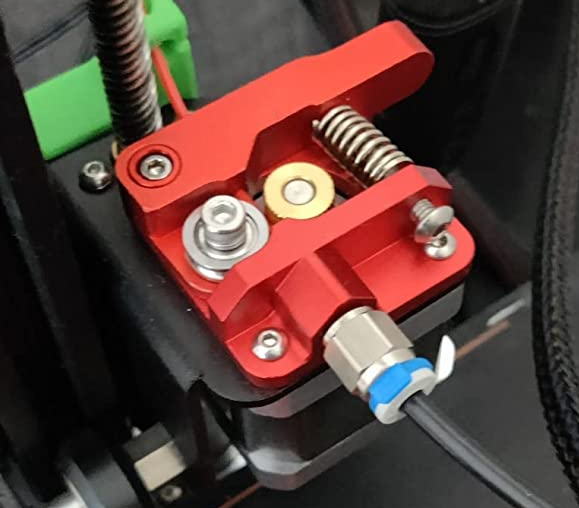
\includegraphics[width=0.4\textwidth]{images/nema17.png}
    \caption{Exemple de mécanisme d'extrusion sur un moteur NEMA 17}
    \label{fig:nema17example}
\end{figure}

\par Ainsi, plusieurs choix sont nécessaires avant d'aboutir à un système abouti : il faut d'abord choisir un moteur pas-à-pas adéquat, ainsi qu'un driver de moteur pas-à-pas compatible, et enfin un mécanisme d'extrusion.

\par Le choix du moteur s'est porté sur un moteur pas-à-pas de la gamme NEMA 17 mentionnée plus haut, en particulier le 42SH38-4A (Figure \ref{fig:42SH38-4A}). Celui-ci peut fournir un couple de $0,36 Nm$, et demande une tension d'alimentation de $2,8 V$ ; raisons pour lesquelles il a été choisi étant donné qu'un grand couple n'est pas nécessaire dans le mécanisme d'extrusion présenté.

\begin{figure}[H]
    \centering
    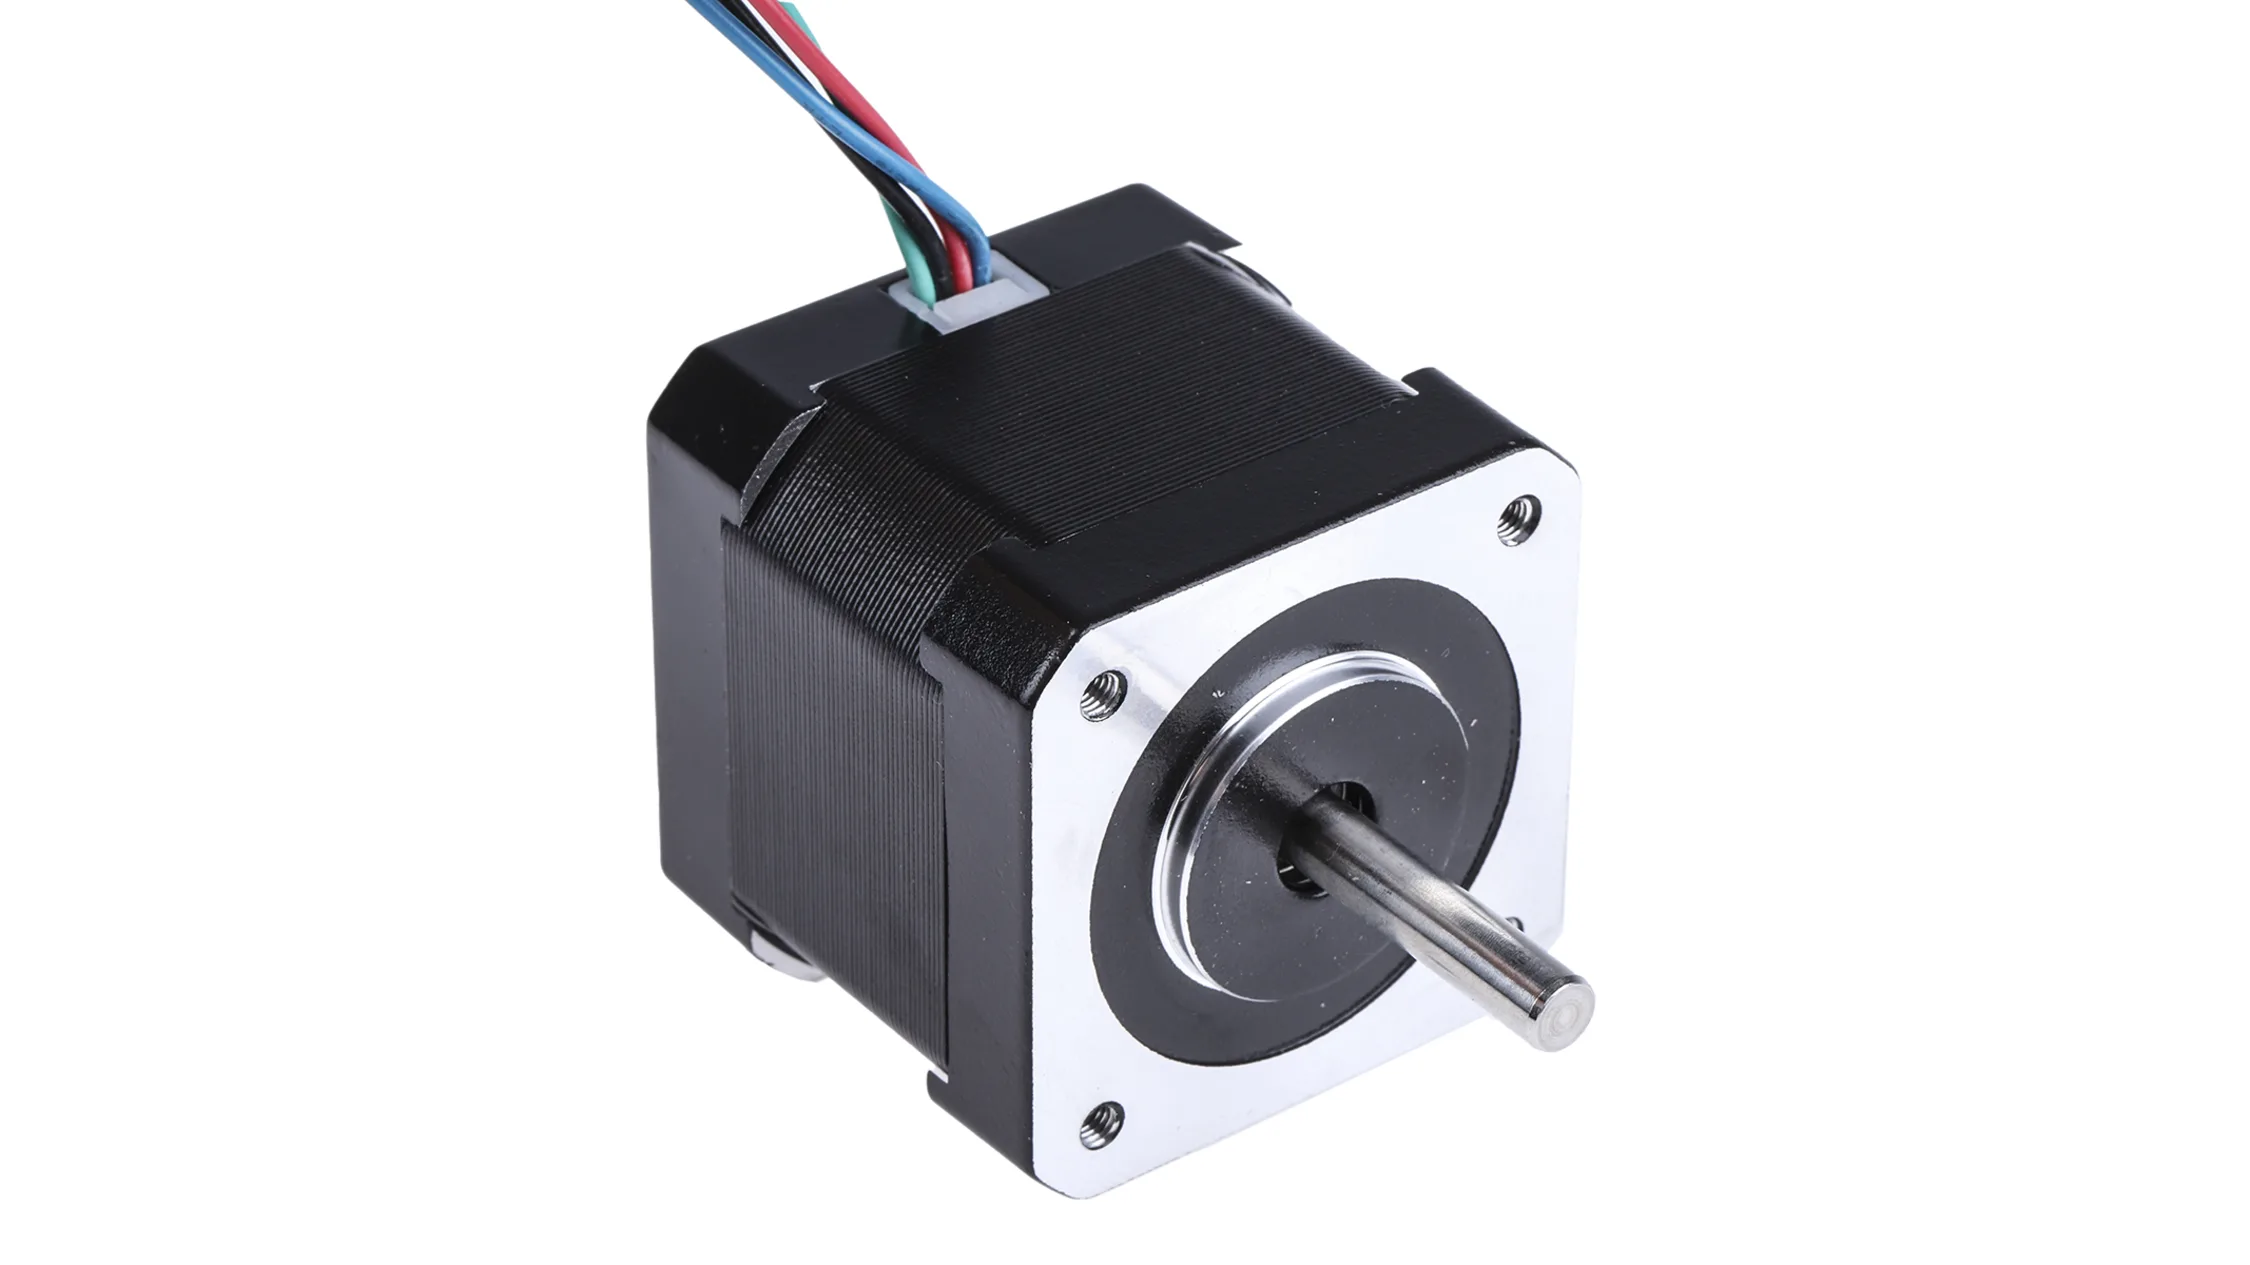
\includegraphics[width=0.5\textwidth]{images/42SH38-4A.png}
    \caption{Moteur pas-à-pas 42SH38-4A}
    \label{fig:42SH38-4A}
\end{figure}

\par Un driver pour moteur pas-à-pas est aussi nécessaire afin de créer le lien entre ce dernier et le microcontrôleur. Ici, c'est le L293D qui est choisi, qui est simplement un composant servant de pont H, permettant de contrôler le moteur pas-à-pas utilisé.

\begin{figure}[H]
    \centering
    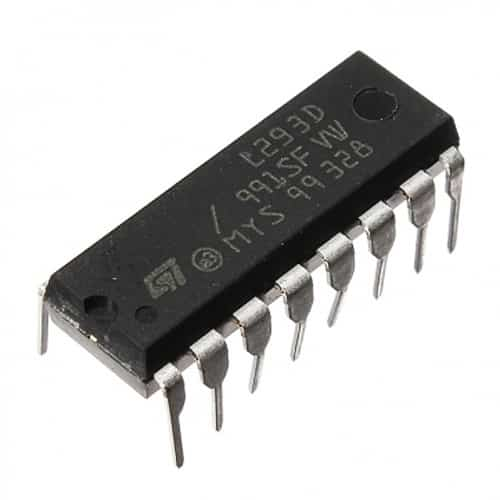
\includegraphics[width=0.2\textwidth]{images/L293D.jpg}
    \caption{Driver pour moteur pas-à-pas L293D}
    \label{fig:L293D}
\end{figure}

\par Enfin, le mécanisme d'extrusion est la dernière pièce nécessaire pour compléter la première partie du projet. En premier lieu, celui-ci avait été modélisé en 3D pour être imprimé et assemblé par la suite. Malheureusement, étant donné un manque d'expérience avec l'impression 3D ainsi que la précision requise pour chacune des pièces, cette idée a dû être abandonnée. Ainsi, des recherches ont été effectuées pour trouver un mécanisme d'extrusion directement prêt à l'achat en ligne ; le choix de celui-ci s'est finalement porté sur l'extrudeuse Bowden de la marque Redrex (Figure \ref{fig:redrex}).

\begin{figure}[H]
    \centering
    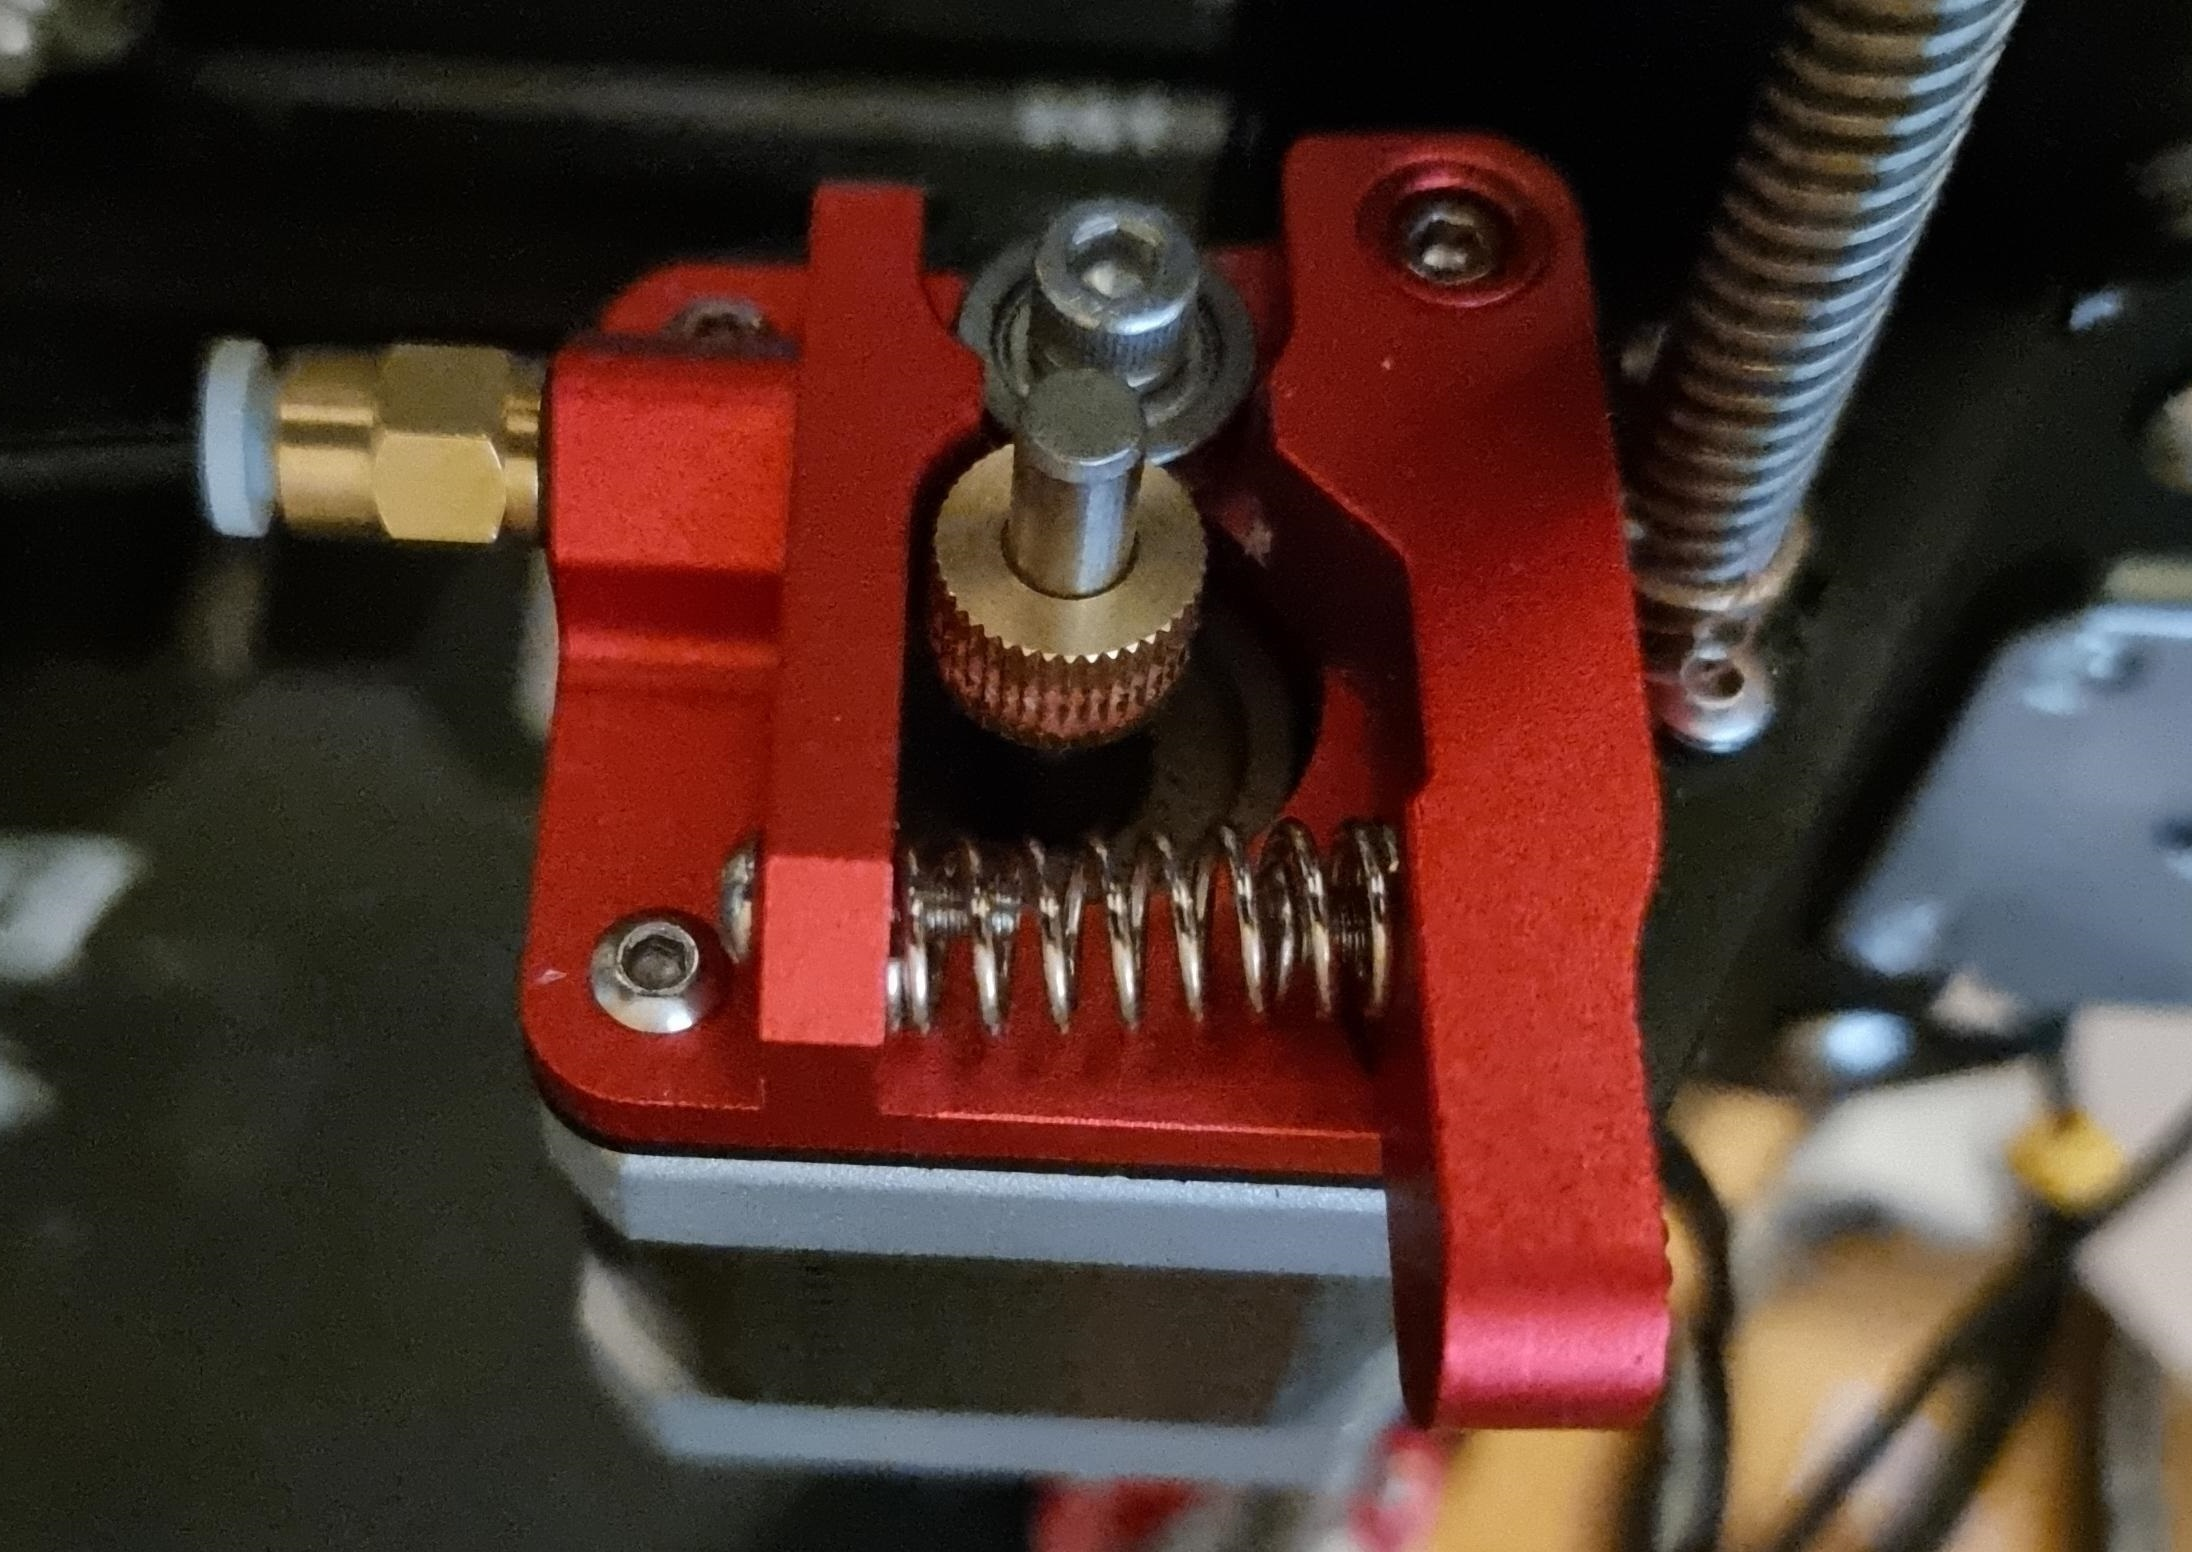
\includegraphics[width=0.4\textwidth]{images/redrex.jpg}
    \caption{Extrudeuse Bowden de la marque Redrex équipée sur un moteur pas-à-pas NEMA 17}
    \label{fig:redrex}
\end{figure}

\par En dernier lieu, un servomoteur est utilisé afin de diriger le fil dans une direction voulue (afin d'éventuellement permettre le choix d'une coupe ou d'un dénudage du fil). Celui-ci est un simple SG90, qui est peu cher et simple d'utilisation. Au final, le servomoteur se trouve dans le prototype, mais n'est pas utilisé étant donné des complications au niveau du dénudage du fil (expliquées dans la prochaine partie du rapport).

\subsection{Coupe du fil}

\par Afin de couper le fil tiré de la manière décrite plus haut, il a été nécessaire de trouver un mécanisme adéquat pour cette partie du prototype. Dans le cas de ce projet, celui-ci se rapproche du système bielle-manivelle : concrètement, le mouvement de rotation d'un moteur pas-à-pas est converti à l'aide de quelques pièces en un mouvement de translation, permettant de contrôler l'ouverture et la fermeture d'une pince pour couper le fil. Ce système convient au prototype et au type du projet pour plusieurs raisons : il est simple à modéliser, ne requiert pas beaucoup de pièces pour être fonctionnel, et, tenant compte d'une bonne construction du mécanisme, il est fiable.

\par Le premier choix à faire était celui de la pince. En effet, avant l'achat de celle-ci, il était important de garder en tête le fait qu'idéalement, le prototype devrait pouvoir couper ou dénuder du fil. C'est pourquoi le choix de la pince s'est porté sur une pince à dénuder multi-fonctions : celle choisie porte en effet des indentations de différentes tailles, permettant notamment le dénudage de fils de certains diamètres, ce qui peut être remarqué dans la Figure \ref{fig:pince}. Un test en magasin avec le fil fourni pour le projet a été fait pour vérifier la compatibilité de la pince. 

\begin{figure}[H]
    \centering
    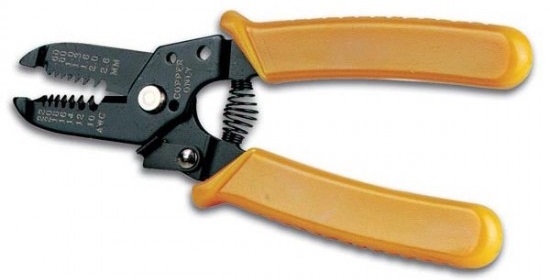
\includegraphics[width=0.6\textwidth]{images/pince.jpg}
    \caption{Pince à dénuder multi-fonctions}
    \label{fig:pince}
\end{figure}

\par En ce qui concerne le moteur pas-à-pas choisi, étant donné qu'un code était fonctionnel pour un autre moteur pas-à-pas de la même gamme dans le prototype et qu'un driver compatible avait aussi été trouvé plus tôt, un NEMA 17 a été choisi, plus particulièrement le 17HS19-2004S1. Il possède des dimensions similaires au 42SH38-4A, mais sa principale différence vient du couple de $0,59 Nm$ qu'il peut fournir. Ceci est important étant donné qu'ici, le couple sera utile pour fournir un réel mouvement dans un système mécanique, contrairement au 42SH38-4A qui était simplement nécessaire pour tirer du fil. Une autre caractéristique importante fut la forme de la tige du moteur : en effet, dans le cas du 17HS19-2004S1, celle-ci est un cylindre tronqué sur sa hauteur. Ceci permet de créer une pièce pouvant s'insérer de manière beaucoup plus stable sur la tige du moteur, ce qui est beaucoup plus difficile sur une tige parfaitement cylindrique, et qui est nécessaire dans le cas du système bielle-manivelle employé ici. Le 17HS19-2004S1 peut être visualisé dans la Figure \ref{fig:17HS19-2004S1}.

\begin{figure}[H]
    \centering
    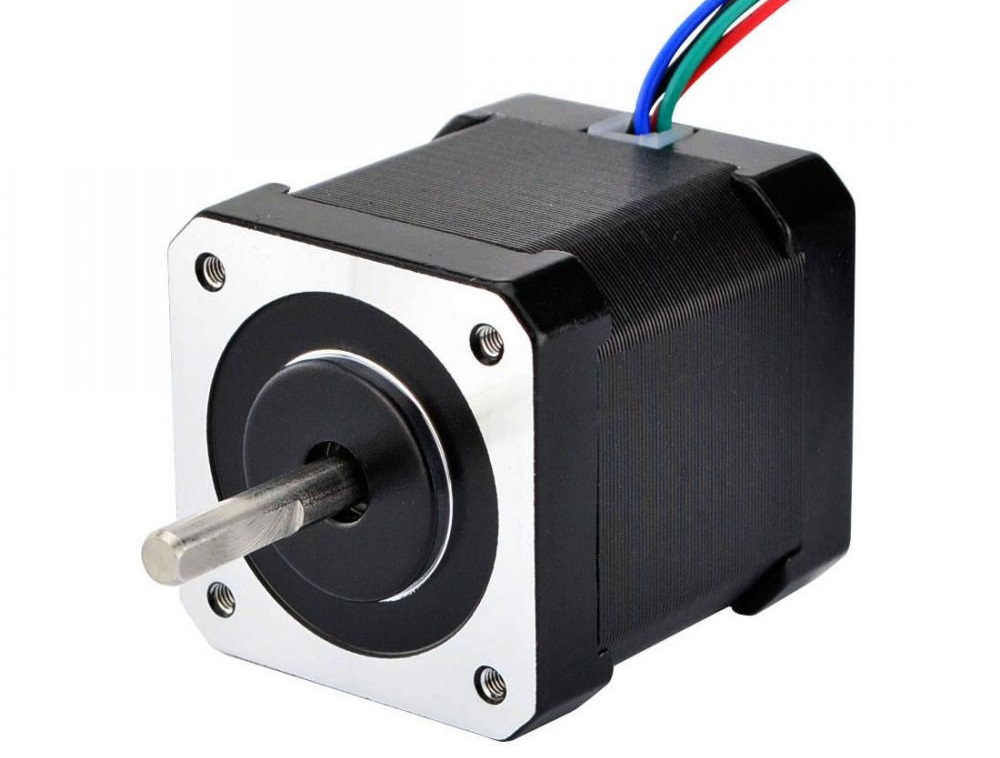
\includegraphics[width=0.4\textwidth]{images/17HS19-2004S1.jpg}
    \caption{Moteur pas-à-pas 17HS19-2004S1}
    \label{fig:17HS19-2004S1}
\end{figure}

\par Ensuite, pour relier le moteur pas-à-pas à la pince, le système bielle-manivelle a dû être modélisé. Ici, il prend forme à l'aide de trois pièces modélisées en 3D :

\begin{itemize}
    \item Un support placé selon la tige du moteur pas-à-pas, avec une indentation circulaire (permettant l'insertion de la manivelle).
    \item Une manivelle en forme de tige surmontée de deux appuis à chacune de ses extrémités.
    \item Un support placé sur une branche de la pince à dénuder, avec une indentation circulaire (permettant l'insertion de la manivelle).
\end{itemize}

Ces trois pièces peuvent être visualisées séparément dans la Figure \ref{figure:piècesbiellemanivelle}.

\begin{figure}[H]
    \centering
    \subfloat[Support du moteur pas-à-pas]{{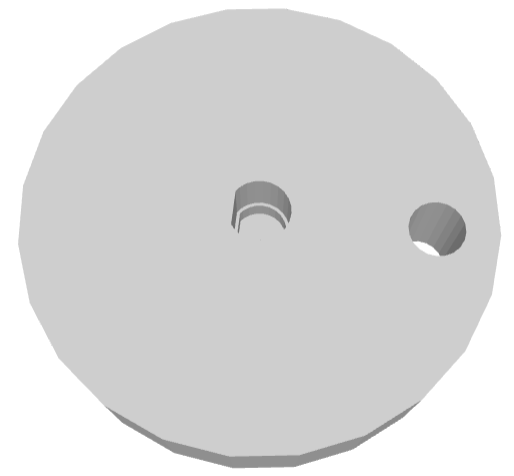
\includegraphics[height=5cm]{images/3Dmoteur}}}
    \qquad
    \subfloat[Manivelle]{{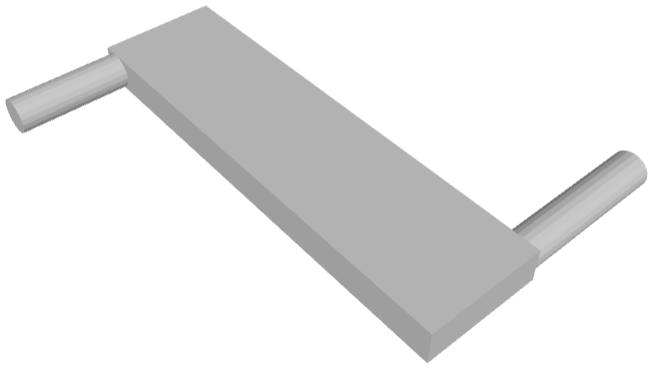
\includegraphics[height=5cm]{images/3Dmanivelle.png}}}
    \qquad
    \subfloat[Support de la pince]{{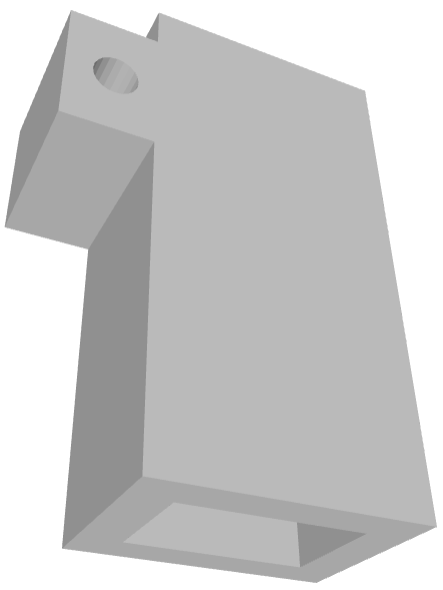
\includegraphics[height=5cm]{images/3Dpince.png}}}
    
    \caption{Pièces modélisées en 3D formant le système bielle-manivelle}
    \captionsetup{justification=centering}
    \label{figure:piècesbiellemanivelle}
\end{figure}

Lorsque ces pièces sont assemblées, le système bielle-manivelle présenté à la Figure \ref{fig:biellemanivelle} est obtenu. Ainsi, le support placé sur le moteur pas-à-pas est fixe dans l'espace, mais peut tourner, ce qui entraîne la manivelle liée au support placé sur la pince. Celle-ci étant elle aussi fixée, ceci permet d'assurer que le support placé ne bougera que verticalement, ouvrant ou fermant ainsi la pince.

\begin{figure}[H]
    \centering
    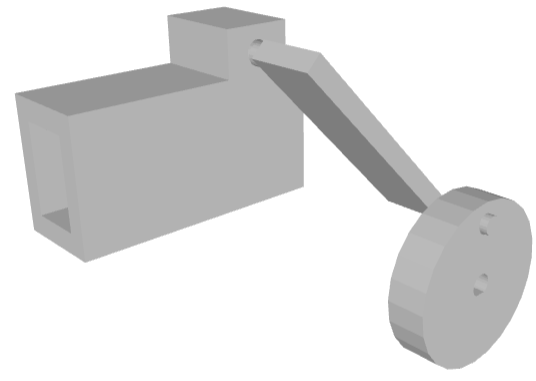
\includegraphics[width=0.6\textwidth]{images/3Dbiellemanivelle.png}
    \caption{Système bielle-manivelle}
    \label{fig:biellemanivelle}
\end{figure}

\par Enfin, le système de coupe de fil obtenu a pu être testé et fonctionne convenablement pour ce but. Malheureusement, l'objectif de pouvoir dénuder du fil n'a pas pu être réalisé : en effet, pour que ceci fonctionne, la position de sortie du fil doit être assez précise pour assurer que celui-ci passera par l'indentation adéquate de la pince à dénuder. Lorsque ce n'est pas le cas, ceci bloque le système bielle-manivelle mentionné, et empêche donc le prototype de fonctionner par la suite.


\subsection{Code et circuit}

\par Le prototype utilise un microcontrôleur fourni par l'ULB pour faire fonctionner le programme principal ; \textit{PSoC Creator} est utilisé pour générer le code en C. Le code créé est surtout utile pour pouvoir gérer les moteurs pas-à-pas dans le prototype ainsi que le servomoteur.

\par Pour les moteurs pas-à-pas, la librairie Arduino pour ce genre de moteurs a été étudiée afin de comprendre la manière de les contrôler (\url{https://github.com/arduino-libraries/Stepper}). Ceci a permis de savoir quelle tension logique appliquer aux broches du moteur pas-à-pas, ainsi que de connaître le sens de ces configurations afin de générer une rotation. Trois fonctions sont donc définies pour chacun des deux moteurs pas-à-pas (d'où la distinction entre \verb|feeder| et \verb|cutter|) : une fonction sert à faire tourner le moteur d'un pas, un autre fait tourner le moteur d'un nombre de pas spécifié en paramètre, et la dernière permet de faire un certain nombre de tours dans le cas du moteur \verb|cutter| ou une certaine distance en mm dans le cas du moteur \verb|feeder| (dans ce dernier cas, il a été mesuré expérimentalement qu'un tour du moteur de tirage faisait avancer $31 mm$ de fil). Dans ces fonctions, un \verb|Timer| est utilisé afin de gérer la fréquence à laquelle les pas sont faits par les moteurs pas-à-pas ; par défaut, cette fréquence vaut $100 Hz$, donc un moteur pas-à-pas peut faire 100 pas par seconde. 

\par Pour le servomoteur, une simple fonction \verb|toggle_servo_position()| est utilisée pour définir si la position du servomoteur devrait permettre la coupe (\verb|SERVO_CUT|) ou le dénudage (\verb|SERVO_STRIP|) du fil. Pour cela, un \textit{pulse-width modulator} (PWM) est utilisé.

\par Le \verb|main()| contient les initialisations des composants, ainsi qu'une boucle infinie du fonctionnement du programme : celui-ci fait simplement tourner le moteur de tirage du fil d'une certaine longueur définie dans le code, puis le moteur de coupe fait une rotation qui permet de couper le fil.

\par Le code source du projet, ainsi que les ressources telles que les fichiers nécessaires à \verb|PSoC Creator| ainsi que les fichiers \verb|.stl| pour les pièces modélisées en 3D se trouvent tous sur le dépôt GitHub suivant : \url{https://github.com/hboughardain/automatic-wire-cutter}. Le code peut aussi être trouvé plus bas dans le rapport au Listing \ref{fig:code}.